% Master File: usersmanual.tex

\chapter{\textsc{The TXTL Modelling Toolbox}}

The TXTL modelling toolbox for MATLAB is a companion to the TXTL Breadboards (Cell-free expression) project being developed at the California Institute of Technology and the University of Minnesota. This toolbox aims to allow \textit{in-silico} prototyping of circuits before they are built \textit{in-vitro}, and to provide insight into circuit behaviour. 

\section{Protocol Overview}

The cell-free circuit breadboard family is a collection of in vitro
protocols that can be used to test transcription and translation
(TX-TL) circuits in a set of systematically-constructed environments
that explore different elements of the external conditions in which
the circuits must operate. This breadboard is based on the work of
Vincent Noireaux at U. Minnesota. The transcription and translation
machineries are extracted from E. coli cells (Shin and Noireaux,
2010). The endogenous DNA and mRNA from the cells are eliminated
during the preparation. The resulting protein synthesis machinery is
used to program cell-free TX-TL gene circuits in reactions of
12uL. The gene circuits can engineered in the laboratory using
standard molecular cloning techniques, but it is also possible to use
PCR products (linear DNA), which substantially decreases the design
cycle time. 

\begin{comment}
\subsection{The TXTL Experimental Protocol}

The endogenous Escherichia coli based TX-TL cell-free expression
system described here is an easy-to-run three-tube reaction that can
take less than 8 hours to set-up, collect, and interpret data. 

\subsection{The TXTL Modelling Protocol}
\end{comment}

The TXTL toolbox commands follow the experimental protocols closely,
and a sample code is given below with brief explanations
of the commands. More detailed explanations can be found in the
'Core Functionalities' chapter. More examples can be found in
the 'Examples' Directory, and are documented in the 'Examples' Chapter
below.

The following code sets up a simple simulation of a negatively
autoregulated gene in the TXTL system (\texttt{negautoreg.m} in the examples directory):
\begin{verbatim}
% Set up the standard TX-TL tubes
tube1 = txtl_extract('E9');
tube2 = txtl_buffer('E9');

% Set up a tube that will contain our DNA
tube3 = txtl_newtube('negautoreg');

dna_tetR = txtl_add_dna(tube3, 'ptet(50)', 'rbs(20)', 'tetR(1200)', 1, 'plasmid');

% Mix the contents of the individual tubes 
Mobj = txtl_combine([tube1, tube2, tube3]);
 txtl_addspecies(Mobj, 'aTc', 600);
 
% Run a simulation
simulationTime = 14*60*60;


tic
[simData] = txtl_runsim(Mobj,simulationTime);
toc
t_ode = simData.Time;
x_ode = simData.Data;

% Plot the results
txtl_plot(t_ode,x_ode,Mobj);
\end{verbatim}
Figure~\ref{fig:intro:negautoreg} shows the output from this code (plotted
using the \url{txtl_plot} function).
\begin{figure}
  \centering
  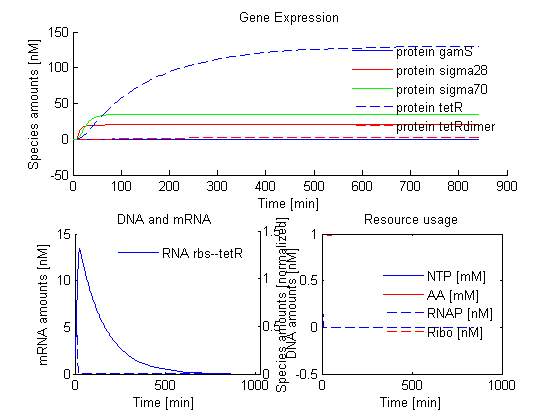
\includegraphics[width=\textwidth]{NegativeAutoregulationPlotActuallyProducedByCode.png}
  \caption{Sample simulation of a negatively autoregulated
  transcriptional circuit.}
  \label{fig:intro:negautoreg}
\end{figure}
